% 2026 University of Pennsylvania PhD Dissertation LaTeX Template v.20260908
% This template aims to fulfill University formatting requirements when one follows the instructions, resolves errors and warnings, and does not edit the style file or font size. Consult https://provost.upenn.edu/for-students/graduate-and-professional-education/graduate-degrees/grad-degrees-faqs/#formattingfaqs for the most up-to-date requirements and policies.
%-------------------------------------------
% We welcome your feedback on the template https://upenn.libwizard.com/f/dissertationlatextemplatefeedback
%-------------------------------------------
% The template is compatable with TeX Live 2026 and optimized for pdfLaTeX and the LaTeX editor Overleaf. Other LaTeX editing programs may require you to compile the document more than once. It is adapted from the Penn Biostat LaTeX Template modified from Dissertation Template for Wharton PhD Candidates in LaTeX. Portions of the text are reprinted or adapted with permission from Ratcliffe SJ. (2017) Penn Biostat LaTeX Template: PhD dissertation.

%%%%%%%%%%%%%%%%%%%%%%%%%%%%%%%%%%%%%%%%%%%%%%%%
%%%%%%%%%%%%%%%%%%%%%%%%%%%%%%%%%%%%%%%%%%%%%%%%
\documentclass[11pt]{report}
\usepackage{upennstyle} % You may add additional packages below this line. Overleaf will warn you if your packages conflict with the template packages. See Chapter 1 for more information.

%-------------------------------------------
% Citation and bibliography commands. Edit as needed.
\usepackage[nonamebreak,round]{natbib}
\bibliographystyle{plainnat}
% \defcitealias{Bodenheimer1986}{BP86}
%-------------------------------------------

%%%%%%%%%%%%%%%%%%%%%%%%%%%%%%%%%%%%%%%%%%%%%%%%
%%%%%%%%%%%%%%%%%%%%%%%%%%%%%%%%%%%%%%%%%%%%%%%%
% PLEASE FOLLOW THE INSTRUCTIONS IN THE CODE COMMENTS
% To uncomment a line of code, remove the % at the beginning of the line
% To comment out a line of code, add a % at the beginning of the line
%%%%%%%%%%%%%%%%%%%%%%%%%%%%%%%%%%%%%%%%%%%%%%%%
%%%%%%%%%%%%%%%%%%%%%%%%%%%%%%%%%%%%%%%%%%%%%%%%

%%%%% PRELIMINARY PAGES %%%%%
%-------------------------------------------
%%%% TITLE PAGE
% Edit the text between curly braces {} relevant to your dissertation.
\title{FROM MASSES TO AGES}
\author{Kaelan Geng}
%\specialization{Field of Specialization} % If you are in Romance Languages or Managerial Science and Applied Economics (Wharton), uncomment this line and edit the text between the {}. If you do, you will also need to edit lines 74 and 75.
\gradgroup{School of Natural Sciences} % See https://provost.upenn.edu/for-students/graduate-and-professional-education/graduate-degrees/graduate-group-coordinators/graduate-groups for names
\date{2026} % Enter current four-digit year
\supervisor{Christian Ginski}
\supervisortitle{Lecturer, School of Natural Sciences}
%\cosupervisor{Co-supervisor's Typed Name} % If applicable, uncomment this line and edit the text between the {}. If you do, you will also need to edit line 39. 
%\cosupervisortitle{Full Faculty Title and Affiliation} % If applicable, uncomment this line and edit the text between the {}. If you do, you will also need to edit line 38.
% \gradchair{Graduate Group Chairperson's Typed Name}
% \gradchairtitle{Full Faculty Title and Affiliation}
% %\cogradchair{Graduate Group Chairperson's Typed Name} % If applicable, uncomment this line and edit the text between the {}. If you do, you will also need to edit line 43.
% %\cogradchairtitle{Full Faculty Title and Affiliation} % If applicable, uncomment this line and edit the text between the {}. If you do, you will also need to edit line 42.
% \committee{Committee Member's Typed Name, Full Faculty Title and Affiliation}
% \committee{Committee Member's Typed Name, Full Faculty Title and Affiliation}
% \committee{Committee Member's Typed Name, Full Faculty Title and Affiliation} % If applicable, comment out or duplicate this line to remove or add a committee member.
%-------------------------------------------

%%%% OPTIONAL COPYRIGHT NOTICE
% \authorlegal{Kaelan Geng} % To opt out of copyrighting your dissertation, uncomment this line. If you do, you will also need to edit line 79.
%-------------------------------------------
%\cclicense{Name of Selected Creative Commons License} % If applicable, uncomment this line and edit the text between the {}. If you do, you will also need to edit lines 54, 79, and 81.
%-------------------------------------------
%\cclicenseurl{URL of selected Creative Commons License} % If applicable, uncomment this line and edit the text between the {}. If you do, you will also need to edit lines 52, 79, and 81.
%-------------------------------------------

%%%% OPTIONAL DEDICATION
% \dedication{Write your dedication text in italics here.} % If not applicable, comment out this line to hide the optional dedication page. If you do, you will also need to edit line 85.
%-------------------------------------------

%%%% OPTIONAL ACKNOWLEDGMENT
% \acknowledgment{Write your acknowledgment text here.} % If not applicable, comment out this line to hide the optional acknowledgment page. If you do, you will also need to edit line 89.
%-------------------------------------------

%%%% ABSTRACT
\abstract{Write your abstract text here.} % Write your abstract between the {}
%-------------------------------------------

%%%% OPTIONAL PREFACE
%\preface{Write your preface text here.} % If applicable, uncomment this line and write your preface between the {}. If you do, you will also need to edit line 104.
%-------------------------------------------

\begin{document}
\maketitle % If you are in Romance Languages or Managerial Science and Applied Economics (Wharton), comment out this line. If you do, you will also need to edit lines 33 and 75.
%\makespecializationtitle % If you are in Romance Languages or Managerial Science and Applied Economics (Wharton), uncomment this line. If you do, you will also need to edit lines 33 and 74.
\setcounter{page}{2}

%%%% OPTIONAL COPYRIGHT NOTICE
% \makecopyright % If not applicable, comment out this line to hide the optional traditional copyright notice page. If you do, you will also need to edit line 50.
%-------------------------------------------
%\makecreativecommons % If applicable, uncomment this line to insert the optional Creative Commons License copyright notice page. If you do, you will also need to edit lines 52, 54, and 79.
%-------------------------------------------

%%%% OPTIONAL DEDICATION PAGE
\makededication % If not applicable, comment out this line to hide the optional dedication page. If you do, you will also need to edit line 58.
%-------------------------------------------

%%%% OPTIONAL ACKNOWLEDGMENT PAGE
\makeacknowledgment % If not applicable, comment out this line to hide the optional acknowledgment page. If you do, you will also need to edit line 62.
%-------------------------------------------

\makeabstract
\tableofcontents

%%%% OPTIONAL LIST OF TABLES
% \clearpage \phantomsection \addcontentsline{toc}{chapter}{LIST OF TABLES} \begin{singlespacing} \listoftables \end{singlespacing}% If not applicable, comment out this line to hide the optional List of Tables
%-------------------------------------------

%%%% OPTIONAL LIST OF ILLUSTRATIONS
\clearpage \phantomsection \addcontentsline{toc}{chapter}{LIST OF ILLUSTRATIONS} \begin{singlespacing} \listoffigures \end{singlespacing}% If not applicable, comment out this line to hide the optional List of Illustrations
%-------------------------------------------

%%%% OPTIONAL PREFACE
%\makepreface % If applicable, uncomment this line to insert the optional preface. If you do, you will also need to edit line 70.
%-------------------------------------------

%%%%% MAIN TEXT %%%%%
\begin{mainf} % The main body of your dissertation starts below this line
\chapter{Introduction}
There is currently no way to systematically determine the age of a planet. In the field of planet formation, the standard practice is assuming coevality: that is, the planet and its host star
are the same age. However, we depend on the age of the planet, along with the luminosity that can be measured from direct imaging, to estimate the mass using evolutionary models. However, it is obvious
that planet formation takes time, possibly millions of years, so it follows that a lot of mass estimates we obtain are based upon incorrect ages. This project aims to tackle this research gap by finding a systematic
method to estimate the age of a planet, using dynamical masses, luminosities from direct imaging and evolutionary models. Before the approach is explored, below is the background required to understand what's required to
undertake this project: how planets form and their respective timescales, how planets are imaged, the aforementioned evolutionary models, a deeper dive into the motivation and then finally the methodology.

% \begin{figure}[H]
% \begin{center}
% 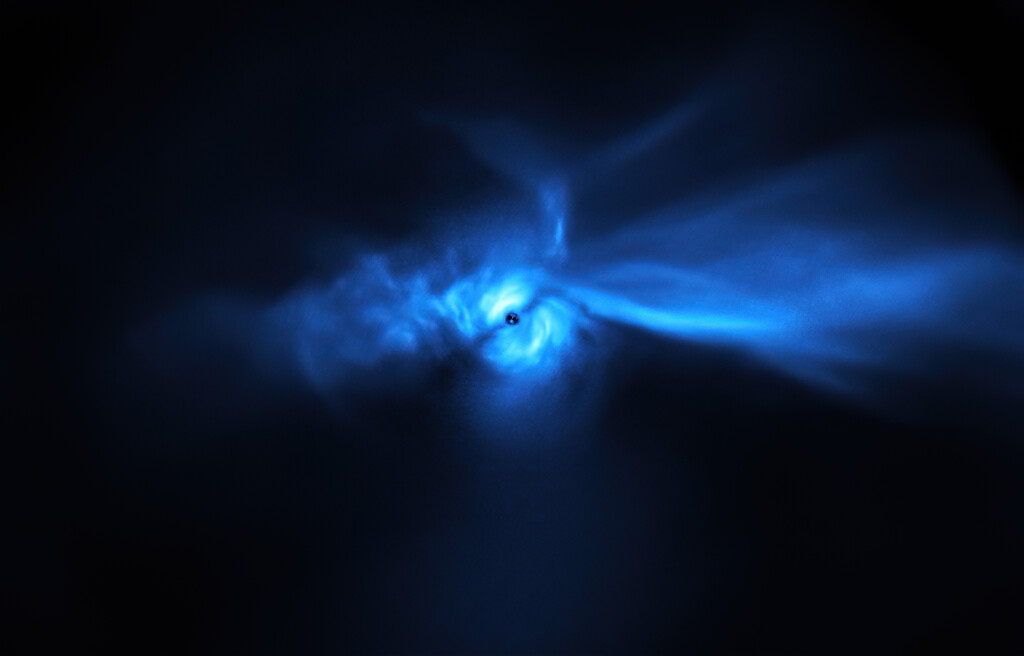
\includegraphics[scale=0.35]{su_aurigae.jpg}
% \caption{The SU Aurigae system. The majority of this photo comprises of wispy arms, which \citealp{Ginski2021} theorise
% is material from the surrounding medium replenishing the material in the disk. Credit: \citealp{Ginski2021}}\label{fig:su_aurigae}
% \end{center}
% \end{figure}

%---------------------------------------------------------------------------------------------------------------------------------

\section{Planetary System Formation}
Planetary systems are born from a planet-forming disk around a young star, which form from a giant molecular cloud ($\sim 10^6M_\odot$, $\sim10^7$ AU) contracting under its own self gravity (\citealp{Shu1987}).
This contraction forms a protostar with a surrounding rotating envelope. Due to the conservation of angular momentum, excess mass from the envelope not accreted by the star will settle into a rotating disk
of gas and dust, which is the planet-forming (protoplanetary) disk of interest. This disk has an expected lifetime of $\sim 10$ Myr (\citealp{Strom1993}), during which it will form planets. Once exhausted of its material,
the disk will dissipate and a planetary system much like our own solar system will result.

%---------------------------------------------------------------------------------------------------------------------------------

\section{Determination of Stellar Age}
The ages of young stars can be determined by a few methods, three of which I will mention in this section as they are of particular relevance to the systems studied in this project.

\subsection{Lithium Depletion Boundary}
This process only happens in groups of stars with the same age, known as moving groups. Young stars contract as they age; in doing so, their core temperatures rise (\citealp{Soderblom2014}). Lithium burning occurs at about $3\times 10^6$ K, and these young stars reach this temperature on a timescale that depends on mass.
We can tell if this has occurred through spectroscopy. The lithium depletion boundary (LDB) is the  between low luminosity stars still have all their lithium, and slightly higher luminosity stars have totally burned through their lithium. 





\subsection{Kinematic Ages}

\subsection{Hertzsprung-Russell Diagrams}

%---------------------------------------------------------------------------------------------------------------------------------


\section{Planetary Formation Mechanisms}
\subsection{Core Accretion}
\begin{sloppypar}
The standard model for gas-giant formation by core accretion comes from \citet{Pollack1996}, 
who built on older accretion models (\citealp{Safronov1969, Mizuno1978, Mizuno1980, Bodenheimer1986}).
A general overview of the process is as follows: a protoplanetary disk consists of dust and gas. 
This dust undergoes random motion, and eventually dust particles may collide and clump together. The repetition of this process eventually leads to pebbles (dust coagulation, \citealp{Drazkowska2023}), 
then boulders, plentesimals, then finally, through planetesimal accretion (\citealp{Safronov1969}), a planetary core massive enough to start accreting gas from the disk, which eventually leads to runaway gas accretion 
(\citealp{Mizuno1980}, \citealp{Bodenheimer1986}, \citealp{Pollack1996}). 

All in all, this process' timescale is on the scale of Myr (\citealp{Pollack1996}), which is significant because a planet formed in this way would be sizeably younger than its host star; planets formed through CA
are also what this project aims to find.
\end{sloppypar}
This process occurs closer to the centre of the disk than gravitational instability, the other widely-accepted formation pathway, detailed in the next section. 
Note that this process is not necessarily linear; most pebbles actually do not evolve to the metre-scale. Among the potential barriers include the fragmentation-barrier, 
drift-barrier and others that are beyond the scope of this project but are detailed in Drazkowska et al. 2023.

\begin{figure}[H]
\begin{center}
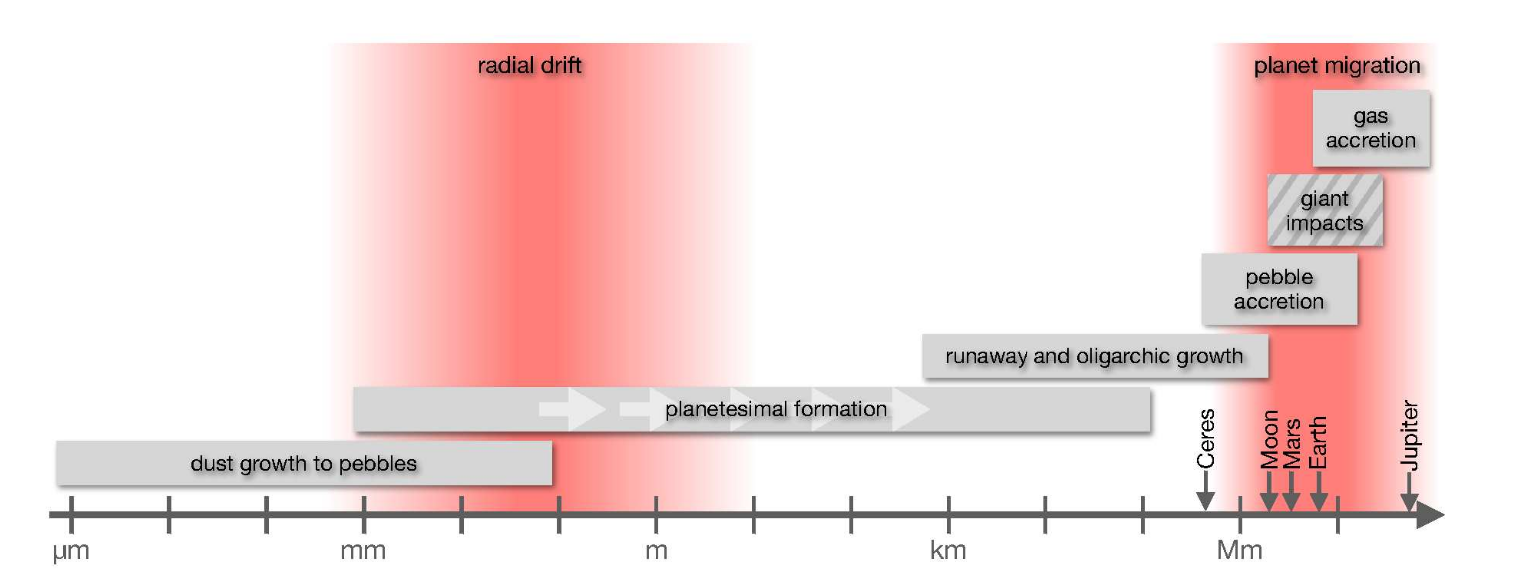
\includegraphics[scale=0.6]{fig3drazkowska2023.png}
\caption{Fig. 3 from Drazkowska2023. This figure provides a general scale for the stages of CA.} \label{fig:fig3drazkowska2023}
\end{center}
\end{figure}

\begin{sloppypar}
Previous models that \citealp{Pollack1996} model built upon include \citealp{Mizuno1978} and \citealp{Mizuno1980} of core instability, \citealp{Bodenheimer1986}'s investigations into Mizuno's models,
\citealp{Pollack1986} and \citealp{Podolak1988} examinations into planetesimal accretion, among others.

In short, a critical mass before runaway gas accretion occurs is found to be $\sim 10M_\oplus$ (\citealp{Mizuno1980}), later $\sim 10M_\oplus - 30M_\oplus$ (BP86), and also when the heavy-element mass
and the gas mass of the planet would equal; after this critical mass is reached, runaway gas accretion occurs. However, observations of the giant planets also revealed that Neptune and Uranus had compositions such that, 
in these models, their mass fractions were comprised of too little gas mass, so they would have never reached the equality required to reach the critical mass. \citealp{Pollack1996}'s remedy to this issue
will be found in the outline below. Note also, that this model occurs after dust and pebble accretion and 
\end{sloppypar}

Arranged neatly, the model of \citealp{Pollack1996} is split into three phases: during phase 1, planetesimal accretion exceeds gas accretion rate;
they're initially many orders of magnitude apart, with planetesimal accretion rate being the greater value. Overtime, the two rates become comparable:
after $\sim 10^5$ years, they are comparable and planetesimal accretion rate begins declining sharply. Meanwhile, gas accretion rate keeps growing.
This phase denotes a runaway planetesimal accretion, separate from the runaway gas accretion, and it finishes when a protoplanet has emptied
its feeding zone of planetesimals. However, the feeding zone grows as the planet's total mass increases, introducing new planetesimals (\citealp{Pollack1996}) 

Phase 2 is a novel phase introduced in this model, that denotes a long, liminal phase where both accretion rates are relatively time-invariant, now with
gas accretion rate exceeding planetesimal accretion rate. This phase spans the bulk of the aforementioned Myr timescale, with Pollack's simulations of Jupiter
lasting $\sim7 Myr$. Finally, phase 3 denotes the runaway gas accretion, where both accretion rates (with gas still far exceeding planetesimal) start rapidly
increasing again.

Fig 1c of \citealp{Pollack1996} is particluarly relevant to this project: during phase 3, the luminosity grows rapidly such that, once fully formed, the planet is bright enough
that we can directly image it. It will then cool down for the rest of its lifetime (since planets have no mechanisms to self-illuminate).

\begin{figure}[H]
\begin{center}
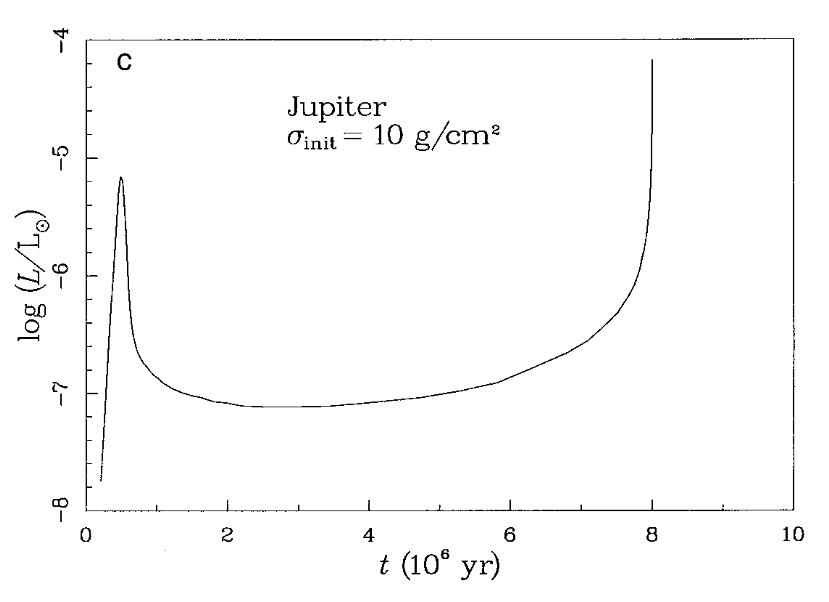
\includegraphics[scale=1.2]{fig1cpollack1996.png}
\caption{Fig 1c of \citealp{Pollack1996}. The initial rise corresponds to the runaway planetesimal accretion of phase 1; the long
plateau corresponds to the transitionary phase 2; the sharp increasing corresponds to both accretion rates rapidly increasing (and the runaway gas accretion)
in phase 3}\label{fig:lum_pollack1996}
\end{center}
\end{figure}

%---------------------------------------------------------------------------------------------------------------------------------

\subsection{Gravitational Instability}
\begin{sloppypar}
Planet formation by gravitational (disk) instability arises in the outer regions of the disk (\citealp{Dodson-Robinson2009}) where it is colder and results from a clump fragmenting from the disk under its own self-gravity.
Its dependence on being cold is due to the Toomre stability criterion Q, given by:
\[
Q = \frac{c_s\Omega}{\pi G \Sigma}
\]
where $c_s$ is the speed of sound, $\Omega$ is rotation frequency, $\Sigma$ is the disk surface density 
(\citealp{Toomre1964,Kratter2016,Longarini2026}). Q determines the stability of a disk: large Q is stable, and $ Q = 1$ is the instability criterion: any $Q < 1 $ is unstable.
The speed of sound scales with temperature, so Q scales linearly with sound speed and thus temperature, and inversely with surface density, so cold massive disks are more prone to instability. The parameters of Q are in a three-way competition:
$\Sigma$ tries to collapse the clump, $c_s$ tries to resist collapse on small scales, $\Omega$ resists on large scales.
\end{sloppypar}
So, instability depends on surface density, rotation and temperature that can create denser regions in the disk, that can then fragment into its own subcloud, which will be contracting. 
This may repeat many times for this fragment, forming sub-subclouds, then sub-sub-sub\ldots clouds (\citealp{Whitworth2006b}). These sub-sub-sub\ldots clouds will contract
continually over a few thousand years to a million years, scaling inversely with mass (so more massive clouds contract faster). Here, the subcloud is made of $H_2$ and is $\sim 10^2$ $R_{Jup}$ in size, 
and will continue to contract, increasing in temperature in the process until a critical temperature of $\sim$ 2000 K (\citealp{Helled2014, Bussmann2026}) is reached, where the $H_2$ dissipates and the now protoplanet undergoes a dynamical collapse, rapidly 
contracting into a dense, compact gas giant of a few $R_{Jup}$. It will then cool in a similar fashion to core accretion.

When observing protoplanetary disks, an indicator of disk instability occurring is spiral arms, characterised by transporting angular momentum throughout the disk, and can be driven by increasing surface density
or decreasing temperature. These formation mechanisms can be seen in Figure~\ref{fig:fig2longarini2026}.
\begin{figure}[H]
\begin{center}
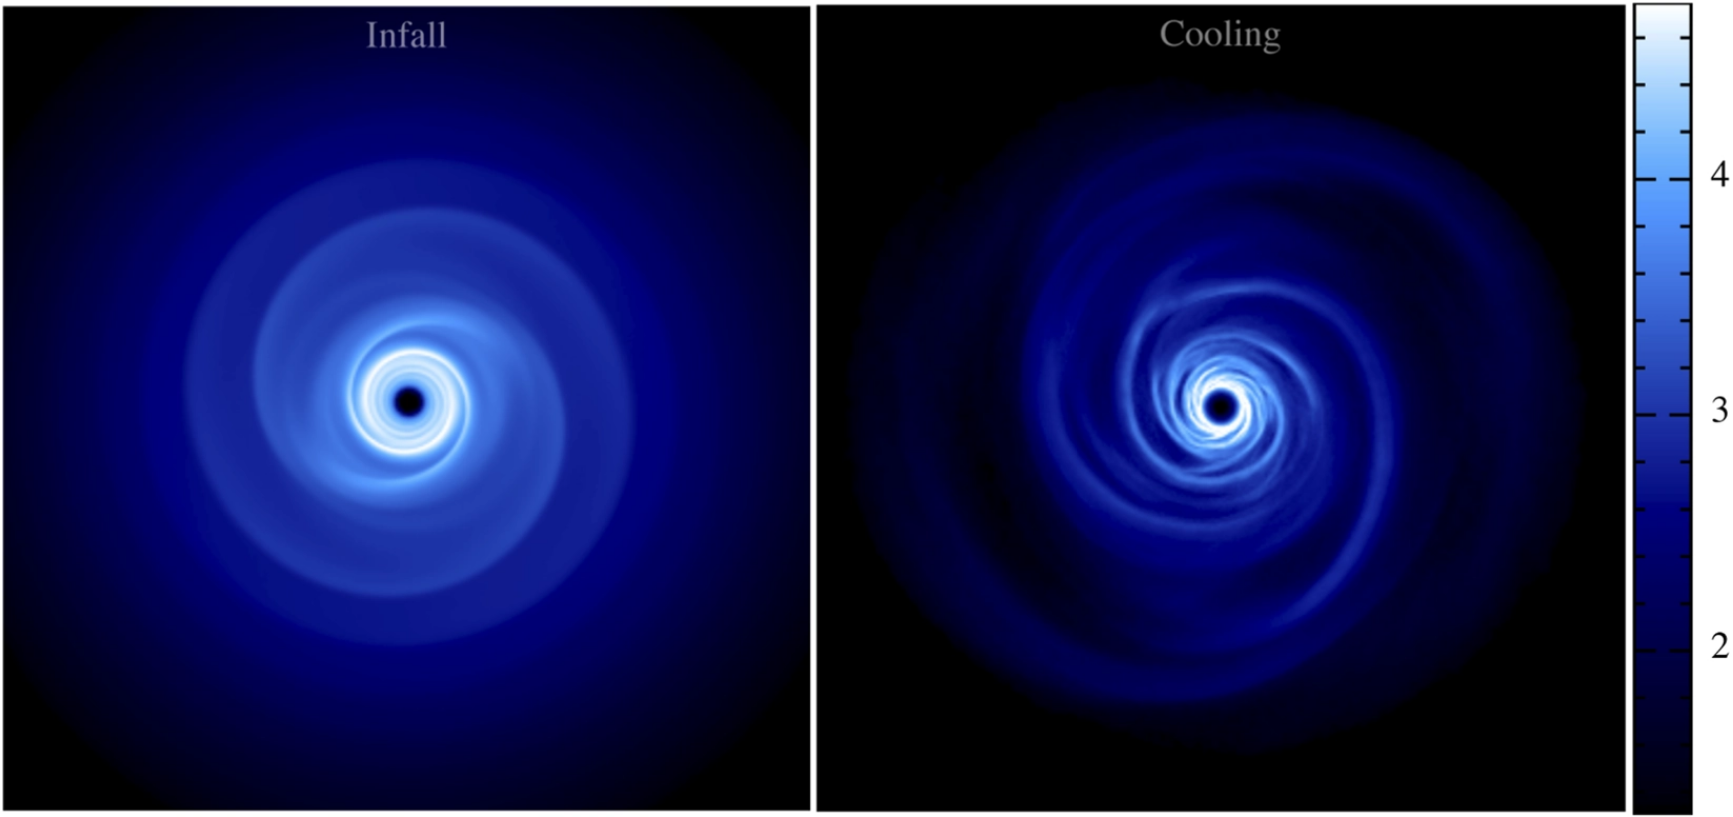
\includegraphics[scale=0.25]{fig2longarini2026.png}
\caption{Fig. 2 from Longarini \& Lodato 2026. It shows two potential transport mechanisms that drive the formation of spiral arms,
where infall is from increasing surface density ($\Sigma$) or cooling (decreasing sound speed $c_s$)}\label{fig:fig2longarini2026}
\end{center}
\end{figure}

\subsection{A Note on Cloud Fragmentation and Brown Dwarfs}
\begin{sloppypar}
Cloud fragmentation is traditionally a mechanism that forms stars. A general overview (see \citealp{Whitworth2006b} for the full process) is that given a molecular cloud is massive enough, it contracts and fragments into subclouds.
This process repeats for the subclouds, until eventually the subclouds are so optically thick that they can't contract anymore since they can't radiate away the contraction heat (\citealp{Whitworth2006b}).

The floor of the mass of objects formed seems to reach well into the planetary-mass range ($\sim$ 1 to 4 $M_{Jup}$, \citealp{Whitworth2006a}).
Also traditionally, the criterion for brown dwarfs is that it exceeds the deterium burning limit of $\simeq 13M_{Jup}$ (\citealp{ChabrierBaraffe2000}), however even this remains challenged;
\citealp{Chabrier2014} argues plantary and brown dwarf can overlap and that there is no clear cut-off mass for one body to be a brown dwarf and another a planet.

Actually, the criterion for what a planet actually is even under debate: some sources base it on only their mass, while some go off the formation tracks. Furthermore, the formation tracks for brown dwarfs are also contested:
many studies theorise that brown dwarfs can form from the low-end masses of cloud fragmentation (\citealp{Balmer2024,Chabrier2003}). Some others suggest they could also be formed through
disk instability (\citealp{Boss1997,Stamatellos2007,Stamatellos2009}) or even core accretion along with the associated runaway gas accretion (\citealp{Balmer2024,DAngelo2010,Molliere2012}).
\end{sloppypar}

Thus, this project will also make use of lower mass brown dwarfs under the assumption that they can use the same formation tracks as planets.

%---------------------------------------------------------------------------------------------------------------------------------

\section{Imaging}
\subsection{Targets}
Most of the planetary systems imaged in this project use the Very Large Telescope (VLT), and the Spectro-Polarimetric High-contrast Exoplanet REsearch (SPHERE) instrument, at the European Southern Observatory.
SPHERE contains the instruments required to carry out the reduction and imaging techniques required to actually observe the planet, such as the coronagraph and wavefront correctors (\citealp{Currie2023}). 
Coronagraphs block out the starlight via physical occulters in the image plane, and deformable mirrors correct for wavefron errors from atmospheric distortion. 

We target young, bright, giant planets at wide orbits because they are luminous enough to actually be imaged, and far enough from their host star that
starlight doesn't obscure the planet and it is detectable within our telescope resolution limits. Binary systems are ignored (\citealp{Currie2023}): they can inhibit planetary formation and disturb planetary orbits due to their chaotic nature. 
In general, the target planets are at separations of 30--300 AU, due to contrast limits at small separations and limited field of view at larger separations.

%---------------------------------------------------------------------------------------------------------------------------------

\subsection{Dynamical Masses}
From imaging, we require the luminosities and dynamical masses from the planets. Dynamical masses are found by fitting the orbits to Kepler's laws through Python packages, e.g., orbitize! (\citealp{Blunt2024}); the separation distance and 
rotation angle from North are required from the orbits.

%---------------------------------------------------------------------------------------------------------------------------------

\section{Evolutionary Models}
Evolutionary models are split into three categories: hot-start, warm-start and cold-start models. 
Hot-start model planets start with high entropy retain high entropy after formation, cold-start models have low entropy, and warm-start models are intermediate between the two former (\citealp{Bowler2016a,Bussmann2026}). 
In the physical world, this translates to core accretion being able to be hot-start or cold-start, depending on how much gravitational energy is radiated away during formation, and gravitational instability heavily faovuring hot-start
due to there being no known mechanism that removes entropy during collapse (\citealp{Galvagni2012,Bussmann2026}). This project will make use of hot-start models in the implementation, due to core accretion not being a favoured formation mechanism
at the studied planets' separations.

%---------------------------------------------------------------------------------------------------------------------------------

\chapter{Motivation}
One of the major caveats to our current models are that planets and their parent stars are not exactly coeval (\citealp{Bowler2016a}). 
Planets can span anywhere from the full stellar age, to 10 Myr younger, depending on the formation mechanism; top-down mechanisms would be close to coeval, while bottom-up mechanisms would leave a discrepancy of a few Myr.
Furthermore, depending on the formation mechanism, it could lead to different inferred masses: take for example the young, planetary-mass companion
2M1207--3932 b of the TW Hydrae Association. Assuming coevality, its hot-start mass is $\sim 5 M_{Jup}$. But, if the formation is delayed by 8 Myr, then
the mass is only $\sim 2.5 M_{Jup}$ (\citealp{Bowler2016a}). Thus, 

%---------------------------------------------------------------------------------------------------------------------------------

\chapter{Literature Review}

%---------------------------------------------------------------------------------------------------------------------------------


\chapter{Methodology}
This project makes use of the species Python package (\citealp{Stolker2020}). The idea is to develop code to brute force an inversion of the evolutionary models, where instead
of getting a mass estimate from age and luminosity, we get an age estimate from the luminosity and dynamical mass. The idea is to create ``standard'' curves, using an evolutionary model (one of ATMO, COND, DUSTY), 
sampling within the uncertainties of the bolometric luminosity of the planet via Monte Carlo sampling and a pre-defined array of ages. The curves will be different for every planet but the implementation is the same.

\begin{figure}[H]
\begin{center}
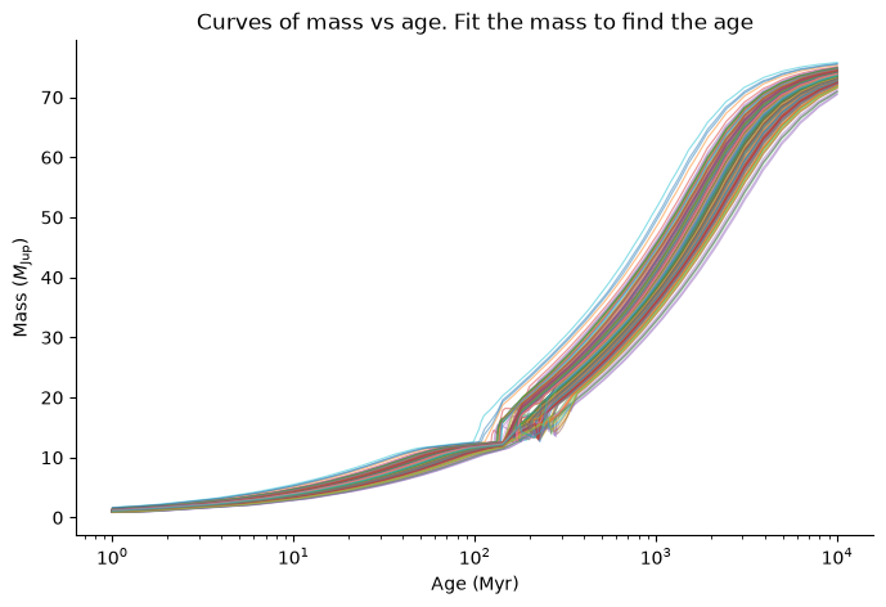
\includegraphics[scale=0.7]{standard curves.png}
\caption{Standard curves for AF Lep b. Generated with $\log{\frac{L}{L_\odot}} = -4.81 \pm 0.13$ and a logspace of ages from 0 to 10 Gyr.}\label{fig:standard}
\end{center}
\end{figure}

The same Monte Carlo sampling is applied to the dynamical mass and its respective uncertainties, which is fitted to the curves via interpolation (see Appendix~\ref{sec:Appendix_A}) to give an age estimate. The median and
first standard deviation is found from this via percentiles.

To include:
- hot-start
- maybe discuss possible solutions and their interpretation

\end{mainf}
%-------------------------------------------

%%%%% OPTIONAL APPENDICES %%%%%
%-------------------------------------------
\begin{append}
\chapter{\MakeUppercase{Interpolation}}
The content of Appendix A begins here. Use the \Verb|\chapter| command to insert additional appendices.
\section{Section Name of Appendix A}\label{sec:Appendix_A}
Use the \Verb|\section| command to create sections.
\end{append}
%-------------------------------------------

%%%%% BIBLIOGRAPHY %%%%%
%-------------------------------------------
\begin{bibliof}
%\nocite{*} % If applicable, uncomment this line to display all entries in the .bib file
\bibliography{bibliography}
\end{bibliof}
%-------------------------------------------
\end{document}